\makeatletter\def\input@path{{Biblio/}{Images/}{Notes/}{Sources/}{Titre/}}\makeatother

\documentclass[a4paper,12pt]{article}
\usepackage[francais]{babel}
\usepackage[utf8]{inputenc}
 
\usepackage{graphicx}
\usepackage{fancybox, fancyhdr}
\usepackage{amsmath, amssymb, amsthm, amsfonts}
\usepackage{chngpage}
\usepackage{listings}
\usepackage{enumerate}
\usepackage{hyperref}
\hypersetup{
    colorlinks,%
    citecolor=black,%
    filecolor=black,%
    linkcolor=black,%
    urlcolor=black
}


%\pagestyle{fancy}

\newcommand{\HRule}{\rule{\linewidth}{0.5mm}}
\theoremstyle{plain}
\newtheorem{theorem}{Théorème}%[section]
\newtheorem{corollaire}{Corollaire}%[section]
\newtheorem{propos}{Proposition}%[section]
\newtheorem{prop}{Propriété}%[section]
\newtheorem{conj}{\textit{Conjecture}}%[section]
%\setcounter{prop}{0} pour réinitialiser le compteur
\theoremstyle{definition}
\newtheorem{defin}{Définition}%[section]
\theoremstyle{remark}
\newtheorem{rmq}{Remarque}%[section]

% début du document --------------------------

\begin{document}
\renewcommand{\chaptername}{} % renome Chapitre en Section

% titre ------------------------------

\begin{titlepage}
\begin{center}

\quad %\\[2cm]
 
\textsc{\Large TER : Coloration de graphes}\\[0.5cm]

\HRule \\[0.5cm]
{ \huge \bfseries Notes}\\[0.4cm]  % <====== IL SUFFIT DE MODIFIER  CE TITRE
 
\HRule \\[1.5cm]

% Author and supervisor
\begin{minipage}{0.4\textwidth}
\begin{flushleft} \large
\emph{Tuteur :}\\
Nadia \textsc{Brauner}
\end{flushleft}
\end{minipage}
\begin{minipage}{0.4\textwidth}
\begin{flushright} \large
\emph{Etudiant :} \\

Michaël \textsc{Gabay}\\
\end{flushright}
\end{minipage}


\quad \\[1.5cm]

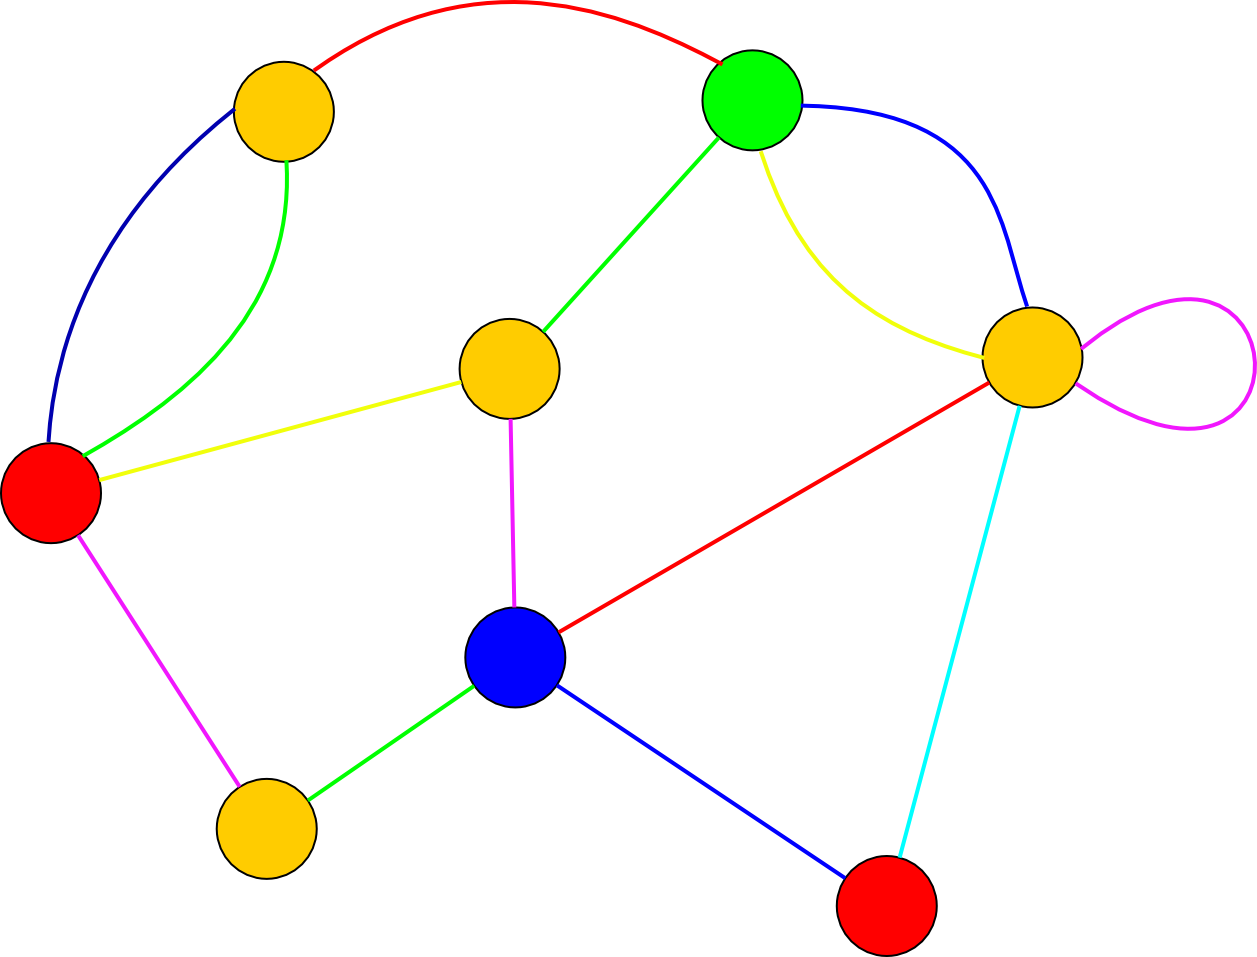
\includegraphics[width=12cm]{graph-color2.png} \\[0.75cm]

\textsc{\LARGE Laboratoire G-SCOP}\\[1.5cm]
%\quad \\[3cm]

\vfill 
% Bottom of the page
{\large Année 2010}

\end{center} 
\end{titlepage}

\changepage	{}%amount added to textheight
           		{4cm}%amount added to textwidth
           		{-2cm}%amount added to evensidemargin
           		{-2cm}%amount added to oddsidemargin
           		{}%amount added to columnsep
           		{}%amount added to topmargin
           		{}%amount added to headheight
           		{}%amount added to headsep
           		{}%amount added to footskip

% tables ------------------------------

\setcounter{page}{1}
\pagenumbering{roman}
\tableofcontents
% \newpage
% \listoffigures
% \newpage
% \listoftables
% \newpage
\pagenumbering{arabic}
\setcounter{page}{1}

% contenu ------------------------------

\begin{titlepage}
\begin{center}

\quad %\\[2cm]
 
\textsc{\Large TER : Coloration de graphes}\\[0.5cm]

\HRule \\[0.5cm]
{ \huge \bfseries Notes}\\[0.4cm]  % <====== IL SUFFIT DE MODIFIER  CE TITRE
 
\HRule \\[1.5cm]

% Author and supervisor
\begin{minipage}{0.4\textwidth}
\begin{flushleft} \large
\emph{Tuteur :}\\
Nadia \textsc{Brauner}
\end{flushleft}
\end{minipage}
\begin{minipage}{0.4\textwidth}
\begin{flushright} \large
\emph{Etudiant :} \\

Michaël \textsc{Gabay}\\
\end{flushright}
\end{minipage}


\quad \\[1.5cm]

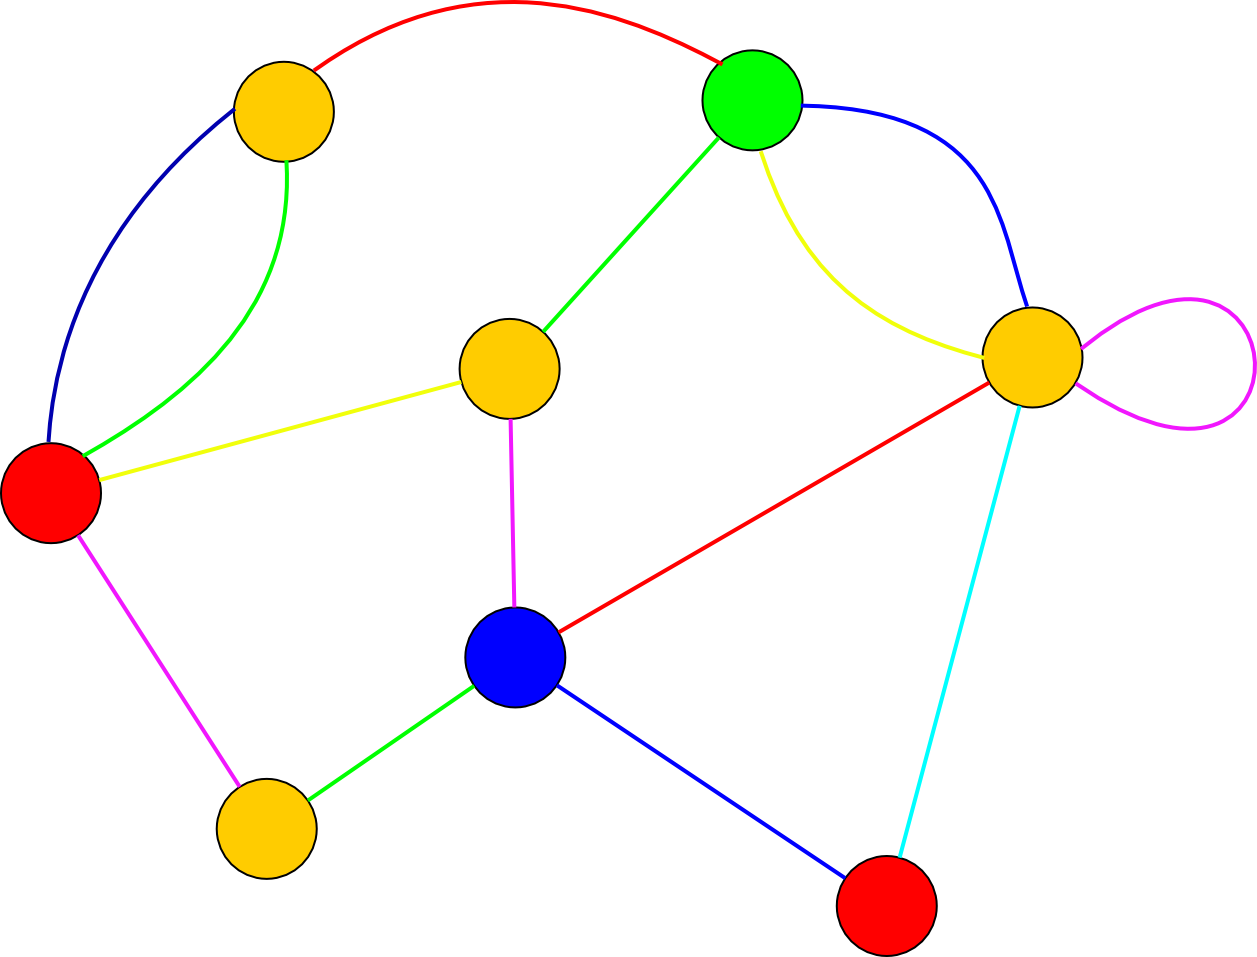
\includegraphics[width=12cm]{graph-color2.png} \\[0.75cm]

\textsc{\LARGE Laboratoire G-SCOP}\\[1.5cm]
%\quad \\[3cm]

\vfill 
% Bottom of the page
{\large Année 2010}

\end{center} 
\end{titlepage}

\changepage	{}%amount added to textheight
           		{4cm}%amount added to textwidth
           		{-2cm}%amount added to evensidemargin
           		{-2cm}%amount added to oddsidemargin
           		{}%amount added to columnsep
           		{}%amount added to topmargin
           		{}%amount added to headheight
           		{}%amount added to headsep
           		{}%amount added to footskip
\clearpage
\section{Idées}
L'identification d'un graphe planaire se fait en $O(n)$ :
\url{http://en.wikipedia.org/wiki/Planarity_testing}\\
La coloration avec 6 couleurs se fait en $O(n)$ (cf \cite{jensen1996graph} p33).\\
La coloration avec 5 couleurs se fait en $O(n^2)$ (cf \cite{jensen1996graph} p33).


% Annexes ----------------------------------------

% \appendix
% \include{append1} => premiere annexe


% Bibliographie ----------------------------------
\nocite{*}
\bibliographystyle{unsrt}
\bibliography{Biblio/biblio}

\end{document}